\documentclass[12pt]{article}

% Настройка русского языка и шрифтов
\usepackage[utf8]{inputenc}
\usepackage[russian]{babel}
\usepackage[T2A]{fontenc}

% Математические пакеты
\usepackage{amsmath, amssymb, amsfonts}

% Настройка страницы
\usepackage{geometry}
\geometry{a4paper, margin=0.8in}

% Другие полезные пакеты
\usepackage{hyperref}
\usepackage{booktabs}
\usepackage{enumitem}
\usepackage{longtable}
\usepackage{graphicx}
\usepackage{xcolor}

% Определение стилей для комментариев
\definecolor{commentgray}{rgb}{0.4,0.4,0.4}
\definecolor{antigravityblue}{rgb}{0.0, 0.45, 0.74}

\newcommand{\commentary}[1]{{\small\itshape\color{commentgray} #1}}
\newcommand{\antigravity}[1]{{\small\color{antigravityblue}\textbf{Antigravity:} #1}}

% Настройка ссылок
\hypersetup{
    colorlinks=true,
    linkcolor=blue,
    filecolor=magenta,      
    urlcolor=cyan,
    pdftitle={Глубокий разбор: Градиентный бустинг (GBDT)},
}


\begin{document}
\maketitle

%\subsection{Фундаментальные основы ансамблей}

\subsection{Дилемма смещения и разброса (Bias-Variance Tradeoff)}
Любую ошибку модели можно разложить на три составляющие:
\[ \text{Error} = \text{Bias}^2 + \text{Variance} + \text{Irreducible Error} \]

\begin{itemize}
    \item \textbf{Bias (Смещение)}: Математическое ожидание разности между истинным ответом и предсказанием. Высокое смещение означает, что модель слишком простая (\textbf{Недообучение}).
    \item \textbf{Variance (Разброс)}: Вариативность предсказаний при смене обучающей выборки. Высокий разброс означает, что модель слишком сложная и подстраивается под шум (\textbf{Переобучение}).
    \item \textbf{Шум (Irreducible Error)}: Ошибка, которую невозможно убрать (ошибки разметки, неполнота данных).
\end{itemize}

\begin{figure}[h]
    \centering
    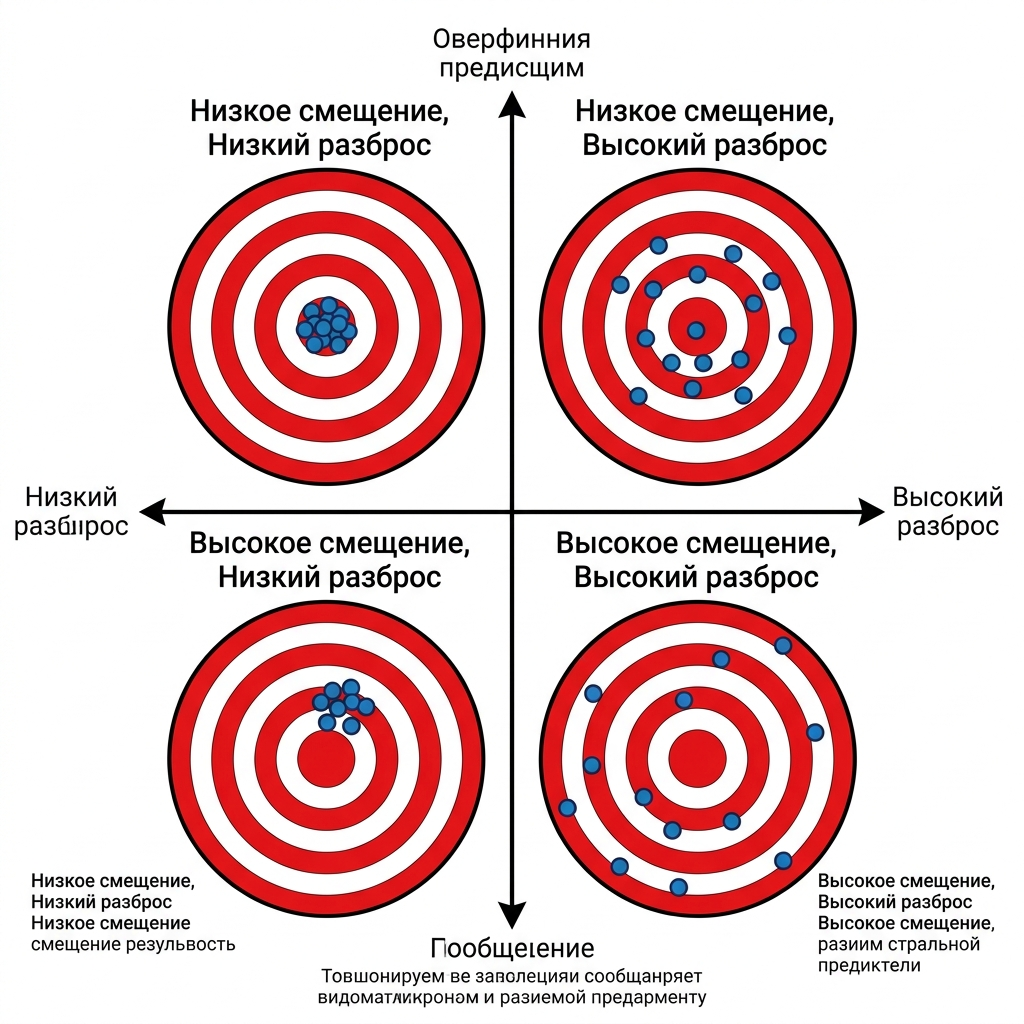
\includegraphics[width=0.8\textwidth]{bias_variance_bullseye.png}
    \caption{Иллюстрация Bias и Variance на примере мишени.}
\end{figure}

\subsection{Случайный лес (Random Forest)}
\textbf{Random Forest} — это ансамбль глубоких решающих деревьев, обученных независимо друг от друга.

\begin{itemize}
    \item \textbf{Как строится (Двойная случайность)}:
    \begin{enumerate}
        \item \textbf{Bagging (Bootstrap Aggregating)}: Каждое дерево обучается на своей подвыборке данных, полученной с помощью бутстрапа (выборка с возвращением). Это дает деревьям «разный взгляд» на данные.
        \item \textbf{Метод случайных подпространств (Feature Subsampling)}: В каждом узле при поиске лучшего сплита дерево выбирает не из всех $D$ признаков, а из случайного подмножества размера $\sqrt{D}$. Это критически важно для \textbf{декорреляции} деревьев.
    \end{enumerate}
    
    \item \textbf{Зачем это нужно?}: Усреднение ответов $N$ независимых моделей с одинаковым матожиданием ошибки сохраняет \textbf{Bias}, но уменьшает \textbf{Variance} в $N$ раз. Чем меньше корреляция между деревьями, тем эффективнее работает ансамбль.
    
    \item \textbf{Минусы}:
    \begin{itemize}
        \item \textbf{Память}: Глубокие деревья занимают очень много места на диске.
        \item \textbf{Скорость}: Работает медленнее бустинга на этапе предсказания (нужно прогнать объект через сотни глубоких деревьев).
        \item \textbf{Экстраполяция}: Как и все деревья, не умеет предсказывать значения вне диапазона обучения.
    \end{itemize}
\end{itemize}

\subsection{Градиентный бустинг (GBDT)}

\subsubsection{Философское отличие: Бустинг vs Бэггинг}
Чтобы понять бустинг, нужно вспомнить случайный лес (бэггинг). 
\begin{itemize}
    \item \textbf{Бэггинг} (Random Forest) строит много глубоких, умных деревьев \textbf{независимо} и усредняет их. Это борется с \textbf{разбросом} (variance).
    \item \textbf{Бустинг} строит цепочку из очень простых («глупых») деревьев \textbf{последовательно}. Каждое следующее дерево исправляет ошибки всех предыдущих. Это борется со \textbf{смещением} (bias).
\end{itemize}

\commentary{Бустинг можно представить как гольфиста, цель которого — загнать мяч в лунку. Здесь положение мяча — ответ композиции. Каждый следующий удар — это та поправка, которую вносит очередной базовый алгоритм. Если гольфист всё делает правильно, то функция потерь будет уменьшаться с каждым ударом.}

\begin{figure}[h]
    \centering
    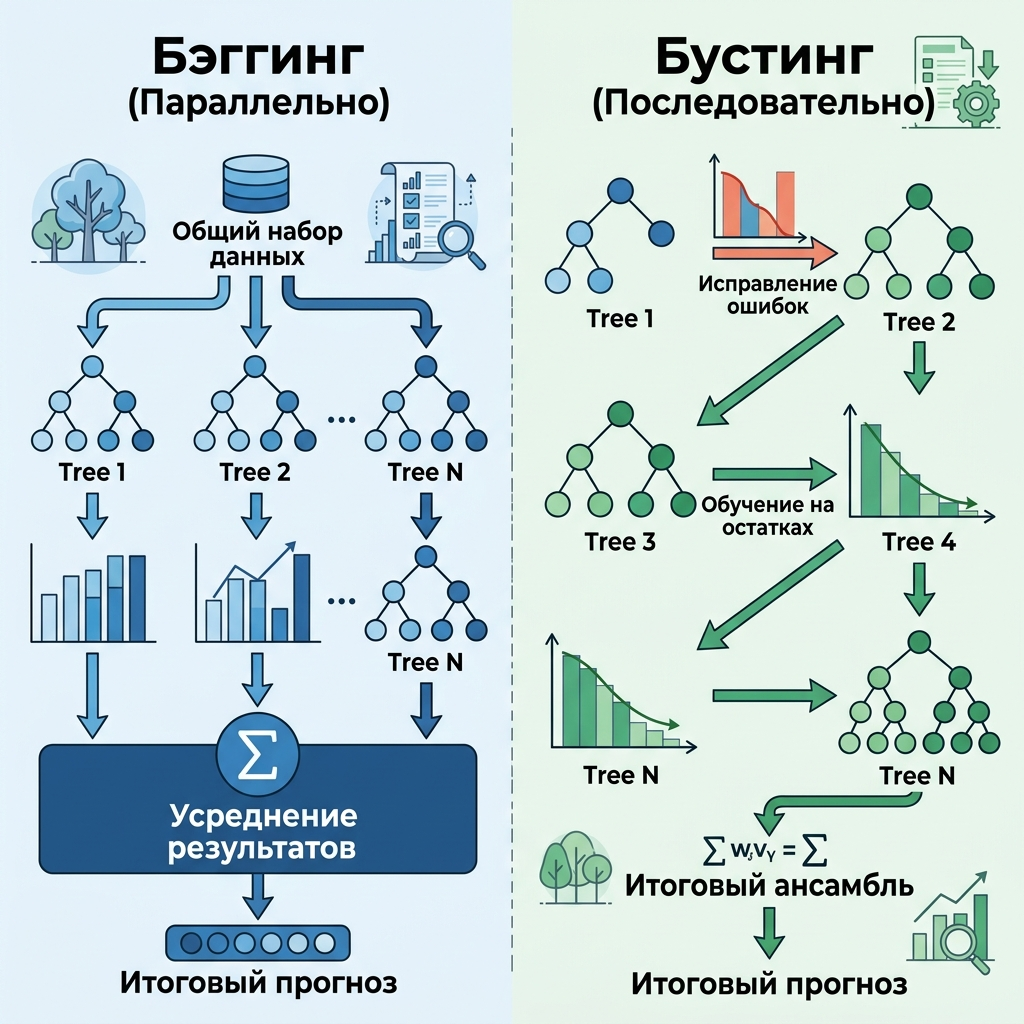
\includegraphics[width=0.7\textwidth]{boosting_bagging.png}
    \caption{Концептуальное различие между Бустингом и Бэггингом.}
\end{figure}

\subsubsection{Математика: Градиентный спуск в функциональном пространстве}

В GBDT мы не подбираем веса объектов или параметры разделяющей поверхности напрямую. Мы ищем саму \textbf{функцию} $f(x)$ в виде суммы базовых алгоритмов, минимизирующую функционал ошибки:
\[ \mathcal{L}(f) = \sum_{i=1}^n L(y_i, f(x_i)) \to \min_f \]

\subsubsection{Алгоритм по шагам}
На шаге $m$ у нас уже есть композиция $f_{m-1}(x) = \sum_{t=1}^{m-1} \eta h_t(x)$. Мы хотим найти такое дерево $h_m(x)$, чтобы:
\[ f_m(x) = f_{m-1}(x) + \eta h_m(x) \]
где $\eta$ — темп обучения (learning rate).

\subsubsection{Почему это градиентный спуск?}
Представим, что мы можем менять предсказания модели в каждой точке $x_i$ независимо. Чтобы минимизировать $L(y_i, f(x_i))$, нам нужно сдвинуть $f(x_i)$ в сторону антиградиента:
\[ f(x_i) \leftarrow f(x_i) - \eta \underbrace{\frac{\partial L(y_i, f(x_i))}{\partial f(x_i)}}_{g_i} \]
Здесь $g_i$ — это \textbf{градиент} функции потерь по предсказанию модели для $i$-го объекта.

\begin{figure}[h]
	\centering
	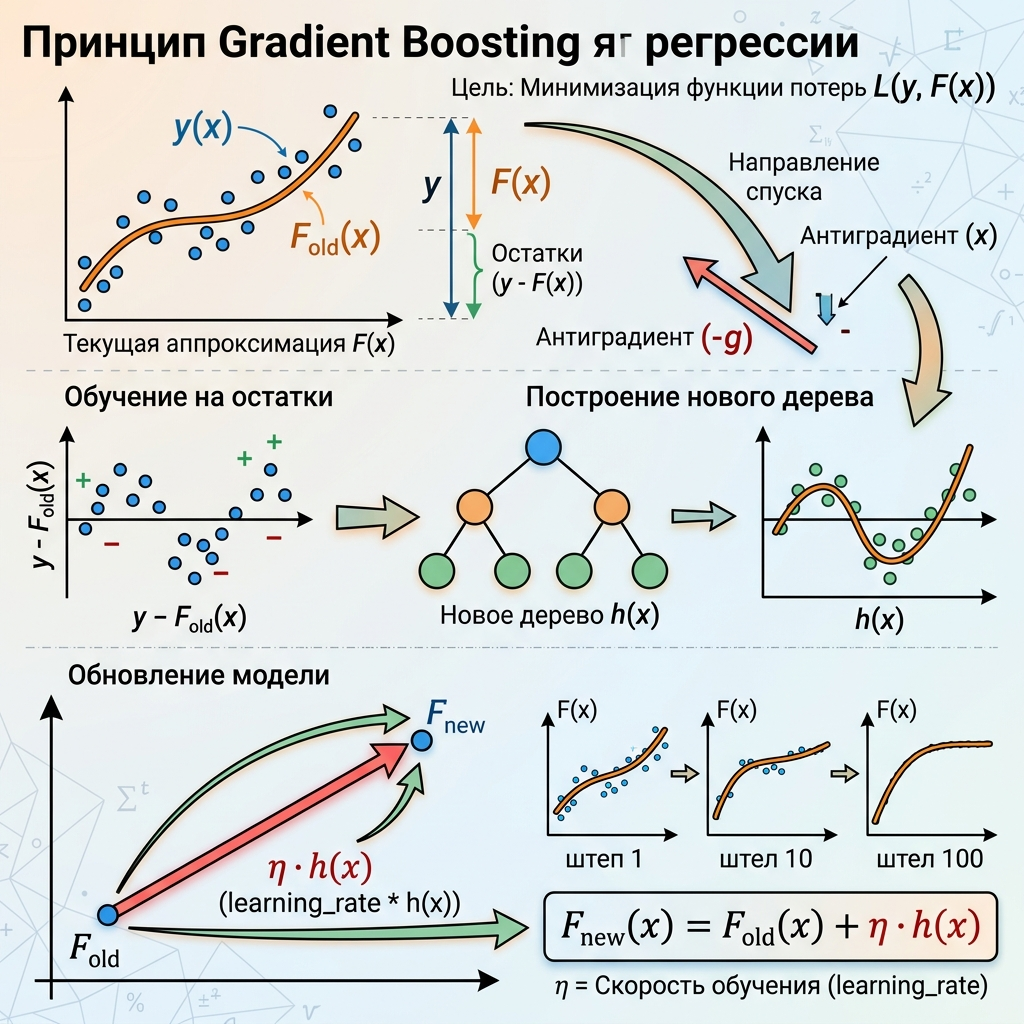
\includegraphics[width=0.7\textwidth]{gbdt_math.png}
	\caption{Процесс обучения нового дерева на антиградиент функции потерь.}
\end{figure}

\subsubsection{Обучение на остатки}
Так как мы ограничены семейством решающих деревьев, мы не можем сделать произвольный сдвиг. Поэтому мы обучаем новое дерево $h_m(x)$ предсказывать значения \textbf{антиградиента} $r_i = -g_i$:
\[ h_m = \arg \min_h \sum_{i=1}^n \left( h(x_i) - r_i \right)^2 \]
Для MSE антиградиент — это просто остатки $(y_i - f_{m-1}(x_i))$. Для других лоссов (например, LogLoss) антиградиент имеет более сложный вид, но логика остается прежней.

\subsubsection{Сходимость}
Метод сходится, потому что на каждой итерации мы добавляем в композицию функцию, которая максимально (в смысле $L_2$) приближает направление наискорейшего спуска в пространстве ответов. Таким образом, с каждым шагом общая ошибка на обучающей выборке гарантированно уменьшается (при достаточно малом $\eta$).

\subsubsection{Ограничение сложности и Регуляризация}
Бустинг по своей природе — очень жадный алгоритм. Если его не ограничивать, он мгновенно «зазубрит» обучающую выборку (переобучится). Для борьбы с этим используются два рычага: ограничение базовых моделей и внешняя регуляризация.

\subsubsection{Почему деревья должны быть неглубокими?}
В отличие от случайного леса, где деревья должны быть глубокими, в GBDT используются «слабые» ученики (обычно глубиной \textbf{3–6 уровней}).
\begin{itemize}
    \item \textbf{Смещение vs Разброс}: Бустинг борется со смещением. Если брать глубокие деревья (у которых разброс и так высокий), ансамбль станет крайне нестабильным.
    \item \textbf{Принцип композиции}: Сила бустинга в \textit{комбинации} тысяч простых правил. Каждое дерево должно вносить лишь небольшое уточнение, исправляя грубые ошибки предыдущих.
    \item \textbf{Взаимодействия}: Дерево глубины $d$ способно уловить взаимодействие (interaction) максимум $d$ признаков. Практика показывает, что взаимодействий 3–6 порядка достаточно для большинства задач.
\end{itemize}

\subsection{Методы борьбы с переобучением (Регуляризация)}
\begin{enumerate}
    \item \textbf{Learning Rate (Shrinkage)}: Мы умножаем предсказание каждого нового дерева на коэффициент $\eta \ll 1$ (например, 0.01). Это заставляет алгоритм «идти к минимуму маленькими шагами», что делает его устойчивым к шуму. Обучение при этом требует больше итераций, но качество на выходе выше.
    
    \item \textbf{Стохастический бустинг (Subsampling)}: Каждое дерево обучается не на всей выборке, а на ее случайном подмножестве (по строкам) или на случайном наборе признаков (по столбцам). Это вносит элемент случайности и мешает деревьям слишком сильно коррелировать между собой.
    
    \item \textbf{Веса листьев (L2 regularization)}: В итоговую функцию потерь добавляется штраф за слишком большие значения в листьях (параметр $\lambda$ в XGBoost). Это делает предсказания деревьев более консервативными.
    
    \item \textbf{Early Stopping (Ранняя остановка)}: Мы прекращаем добавлять новые деревья, когда ошибка на \textbf{валидационной} выборке перестает падать. Это самый эффективный способ найти оптимальное количество итераций $M$.
\end{enumerate}

\subsection{Тройка лидеров: XGBoost, LightGBM, CatBoost}

Каждая из этих библиотек — это эволюция классического GBDT, решающая проблемы скорости, памяти и качества.

\subsubsection{XGBoost (eXtreme Gradient Boosting)}
Первый массовый лидер, который принес бустингу популярность на Kaggle.
\begin{itemize}
    \item \textbf{Как строится}: Использует \textbf{Level-wise} рост (дерево растет по уровням, сохраняя баланс).
    \item \textbf{Математическая фишка}: Аппроксимация функции потерь рядом Тейлора до \textbf{второго порядка} (использует и градиент, и \textbf{гессиан} — вторую производную). Это позволяет точнее находить направление спуска.
    \item \textbf{Плюсы}:
    \begin{itemize}
        \item \textbf{Sparsity-aware}: Умеет эффективно обрабатывать пропуски (направляет их в «лучшую» сторону при сплите).
        \item \textbf{Регуляризация}: Встроенные L1 и L2 штрафы прямо в функции поиска сплита.
    \end{itemize}
\end{itemize}

\subsubsection{LightGBM (от Microsoft)}
Создан для работы с \textbf{Big Data}. Когда данных миллионы, XGBoost становится слишком медленным.
\begin{itemize}
    \item \textbf{Как строится}: \textbf{Leaf-wise} рост (разбивает тот лист, который дает максимальное падение лосса, независимо от уровня). Деревья могут быть очень глубокими и асимметричными.
    \item \textbf{Математические фишки}: 
    \begin{itemize}
        \item \textbf{GOSS}: Отбрасывает объекты с маленькими градиентами (на них модель уже выучилась) и оставляет только «сложные».
        \item \textbf{EFB}: Объединяет взаимоисключающие признаки в один (актуально для разреженных данных).
    \end{itemize}
    \item \textbf{Плюсы}: Экстремальная скорость и низкое потребление памяти.
\end{itemize}

\subsubsection{CatBoost (от Яндекса)}
Король табличных данных с большим количеством категориальных признаков.
\begin{itemize}
    \item \textbf{Как строится}: \textbf{Symmetric Trees} (Oblivious Trees). На каждом уровне дерева используется один и тот же признак и один и тот же порог для всех узлов. Это работает как очень сильная регуляризация.
    \item \textbf{Математические фишки}: 
    \begin{itemize}
        \item \textbf{Ordered Boosting}: Решает проблему «смещения предсказания» (prediction shift), обучая модели на перестановках данных.
        \item \textbf{Native Categorical Support}: Использует продвинутую версию Target Encoding, которая не приводит к утечке данных.
    \end{itemize}
    \item \textbf{Плюсы}: Минимум тюнинга «из коробки», лучшая точность на категориях, очень быстрый инференс (из-за симметрии деревьев).
\end{itemize}

\begin{table}[h]
    \centering
    \small
    \begin{tabular}{@{}llll@{}}
        \toprule
        \textbf{Параметр} & \textbf{XGBoost} & \textbf{LightGBM} & \textbf{CatBoost} \\
        \midrule
        Рост дерева & Level-wise & Leaf-wise & Symmetric \\
        Скорость & Средняя & Высокая & Средняя (на обучении) \\
        Категории & One-Hot / Числа & Индексация & \textbf{Native (Best)} \\
        Пропуски & Авто-направление & Авто-направление & Режим "Min/Max" \\
        \bottomrule
    \end{tabular}
    \caption{Сравнение ключевых характеристик библиотек бустинга.}
\end{table}

\subsection{Интерпретация: Feature Importance}
Понимание того, почему модель приняла решение, не менее важно, чем сама точность. В бустинге есть три основных способа оценить важность признаков.

\begin{enumerate}[label=\arabic*., leftmargin=*]
    \item \textbf{Weight / Frequency (Частота)}
    \begin{itemize}
        \item \textbf{Суть}: Считает, сколько раз данный признак был выбран для разделения (сплита) во всех деревьях ансамбля.
        \item \textbf{Минусы}: Очень \textbf{ненадежный} метод. Он поощряет непрерывные признаки с большим количеством уникальных значений (например, ID или случайный шум), так как дерево может «пилить» их бесконечное число раз. При этом реальный вклад в точность может быть нулевым.
    \end{itemize}

    \item \textbf{Gain (Прирост)}
    \begin{itemize}
        \item \textbf{Суть}: Суммирует вклад каждого признака в уменьшение функции потерь (Gain) во всех узлах, где он использовался.
        \item \textbf{Плюсы}: Самый популярный встроенный метод. Он показывает, насколько реально «помог» признак снизить ошибку.
        \item \textbf{Минусы}: Всё еще может быть смещен в сторону признаков с высокой кардинальностью (много категорий).
    \end{itemize}

    \item \textbf{Permutation Importance (Важность через перемешивание)}
    \begin{itemize}
        \item \textbf{Суть}: Мы берем отложенную выборку, замеряем качество. Затем перемешиваем значения одного признака (разрушая его связь с таргетом) и смотрим, насколько упала метрика. Чем сильнее падение — тем важнее признак.
        \item \textbf{Плюсы}: \textbf{Самый честный} метод. Он не зависит от структуры дерева и показывает реальную ценность признака для предсказательной силы на новых данных.
        \item \textbf{Минусы}: Требует много времени на вычисления (нужно прогонять предсказания много раз). Плохо работает, если признаки сильно коррелируют между собой.
    \end{itemize}
\end{enumerate}

\antigravity{На практике всегда смотри на \textbf{Gain}, но проверяй его через \textbf{Permutation Importance} или \textbf{SHAP values}. Если признак имеет высокий Gain, но нулевой Permutation — скорее всего, модель нашла в нем шум или «чит», который не работает на новых данных.}

\vspace{1cm}
\commentary{Главное при работе с бустингом — следить за графиком лосса на валидации. Как только ошибка на валидации перестала падать, а на трейне продолжает — немедленно останавливайся (это называется Early Stopping).}

\antigravity{Для большинства табличных задач CatBoost — это выбор по умолчанию благодаря отличной работе с категориями и регуляризации.}

\end{document}
